\chapterimage{chapter_head_2.pdf} % Chapter heading image

\chapter{Minimização do erro em funções: $\mathbb{R}$ $\rightarrow$ $\mathbb{R}$}

%%%%%%%%%%%%%%%%%%%%%%%%%%%%%%%%%%%%%%%%%%%%%%%%%%%%%%%%%%%%%%%%%%%%%%%%%%%%%%%%%%%%%%%
%%%%%%%%%%%%%%%%%%%%%%%%%%%%%%%%%%%%%%%%%%%%%%%%%%%%%%%%%%%%%%%%%%%%%%%%%%%%%%%%%%%%%%%
%%%%%%%%%%%%%%%%%%%%%%%%%%%%%%%%%%%%%%%%%%%%%%%%%%%%%%%%%%%%%%%%%%%%%%%%%%%%%%%%%%%%%%%
\section{Minimização de $||h(x)-a||^2$} 

\begin{theorem}[Solução iterativa]\label{theo:minhxhx}
Dados,
um escalar $x \in \mathbb{R}$, 
um escalar $a \in \mathbb{R}$,  
uma função $h:\mathbb{R} \rightarrow \mathbb{R}$, e 
definida a Eq. (\ref{eq:minhxhx1}),
\begin{equation}\label{eq:minhxhx1}
e(x)=||h(x)-a||^2.
\end{equation}

Se desejamos ter o valor $\hat{x}$ que minimiza o escalar $e(\hat{x})$,
este valor pode ser achado usando iterativamente a Eq. (\ref{eq:minhxhx2}),
onde  $h'(x)\equiv \frac{\partial h(x)}{\partial x}$.
\begin{equation}\label{eq:minhxhx2}
x_{k+1} \leftarrow x_k-
\frac{ h(x_k)-a}{h'(x_k)},
\end{equation}


Assim, $\hat{x}$ pode ser achado iniciando a Eq. (\ref{eq:minhxhx2}) desde um 
$x_{0}$ qualquer, 
\begin{itemize}
    \item ate que $x_{k}$ seja muito próximo a $x_{k-1}$ (convergência de $x_{k}$) ou
    \item ate que $h(x_{k})$ seja muito próximo a $a$, 
    se conhecemos que esta igualdade é possível,
\end{itemize}
onde pode ser declarado que $\hat{x} \approx x_{k}$.\\

No processo de busca, podemos ter 3 diferentes casos:
\begin{itemize}
\item \textbf{Quando $x_{k}$ converge:}  
Se a Eq. (\ref{eq:minhxhx2}),  converge a um valor $\hat{x}$, então este se trata de 
um mínimo absoluto de
$e(x)$, ou seja $\hat{x}\approx x_k\approx x_{k-1}$, ver Prova \ref{proof:theo:minhxhx} e Exemplos \ref{ex:minhxhx} e \ref{ex:minhxhx3}.

\item \textbf{Quando $x_{k}$ diverge:}  
Acontece quando se tem passado por
um valor de $x_k$ com $0 <|h'(x_k) | < \lim\limits_{\varepsilon \rightarrow +0}\varepsilon$. 
Esta característica da Eq. (\ref{eq:minhxhx2}) é um problema, quando o mínimo valor de $e(x)$ coincide
com um lugar onde $h'(x) = 0$, ver Exemplo \ref{ex:minhxhx}; pois quando se está perto
da solução a busca diverge.

\item \textbf{Quando é não computável:} 
Sim se obtêm um ponto $x_k$ onde $h'(x_k) = 0$,
deve ser verificado se $e(x_k)$ é um mínimo, um
máximo, relativo ou absoluto, ou um ponto de inflexão. \\
\end{itemize}

Para reconhecer o tipo de ponto crítico de $e(x)$, e souber se 
a busca debe ser continuada desde outro ponto, 
podemos seguir vários procedimentos; por exemplo, estudar o comportamento 
de $e(x_k)$ e/ou analisar  $\frac{\partial^2 e(x)}{\partial x^2}$ avaliada em $x_k$.

Uma forma de iterar, como a vista na Eq (\ref{eq:minhxhx2}) é conhecida como método de Newton,
porem pela forma de como esta expressão foi deduzida também poderíamos ligar esta ao
método de regularização de Tikhonov.
A demostração da Eq (\ref{eq:minhxhx2}) pode ser vista na Prova \ref{proof:theo:minhxhx}.
\end{theorem}



\begin{example}\label{ex:minhxhx}
 A Fig. \ref{fig:hxacasesa} nos mostra o processo de busca de um mínimo
 de $e(x)=(h(x)-a)^2$, quando $h(x)=x^2$ e $a=1$. A busca inicia em $x_0=-1.5$,
 todos os valores $x_{k}$ podem ser vistos na segunda coluna da
Tabela \ref{tab:hxacases}. Neste caso a Eq. (\ref{eq:minhxhx2}) \textbf{converge} sem problemas em $\hat{x}=-1$ com $e(\hat{x})=0$,
 pois no caminho não foi achado nenhum ponto $x_{k}$ com $h(x_{k})\cong 0$.

 Por outro lado, a Fig. \ref{fig:hxacasesb} nos mostra o processo de busca de um mínimo
 de $e(x)=(h(x)-a)^2$, quando $h(x)=x^2$ e $a=-1$. A busca inicia em $x_0=-1.5$,
 todos os valores $x_{k}$ podem ser vistos na terceira coluna da
Tabela \ref{tab:hxacases}. Neste caso a Eq. (\ref{eq:minhxhx2}) \textbf{diverge} 
em $\hat{x}=0$ com $e(\hat{x})=0$ que é o mínimo;
ao principio os valores de $x_{k}$ tendem a procurar o mínimo; porem,
perto de este valor se cumpre que $h(x_{k})\cong 0$, e o valor de $x_{k}$ diverge
a um valor muito longe do mínimo; é fácil de observar, que neste caso se produz 
uma especie de efeito sanfona, onde $x_{k}$ se aproxima ao mínimo $e(x)$, e quando 
está perto do mínimo o valor volta divergir.
\begin{table}[!h]
\centering
\begin{tabular}{|l|l|l|}
\hline
~&$e(x)=(x^2-1)^2$ & $e(x)=(x^2+1)^2$ \\ \hline
$k$&$x_k$  & $x_k$ \\ \hline
0&-1.5000  & -1.5000      \\
1&-1.0833  & -0.41667     \\
2&-1.0032  & +0.99167     \\
3&-1.0000  & -0.0083683   \\
4&-1.0000  & +59.745      \\  \hline
\end{tabular}
\caption{Convergência para $h(x)=x^2$ da equação iterativa do Teorema \ref{theo:minhxhx}}
\label{tab:hxacases}
\end{table}
\end{example}

\begin{figure}[!h]
    \centering
    \begin{subfigure}[b]{0.45\textwidth}
        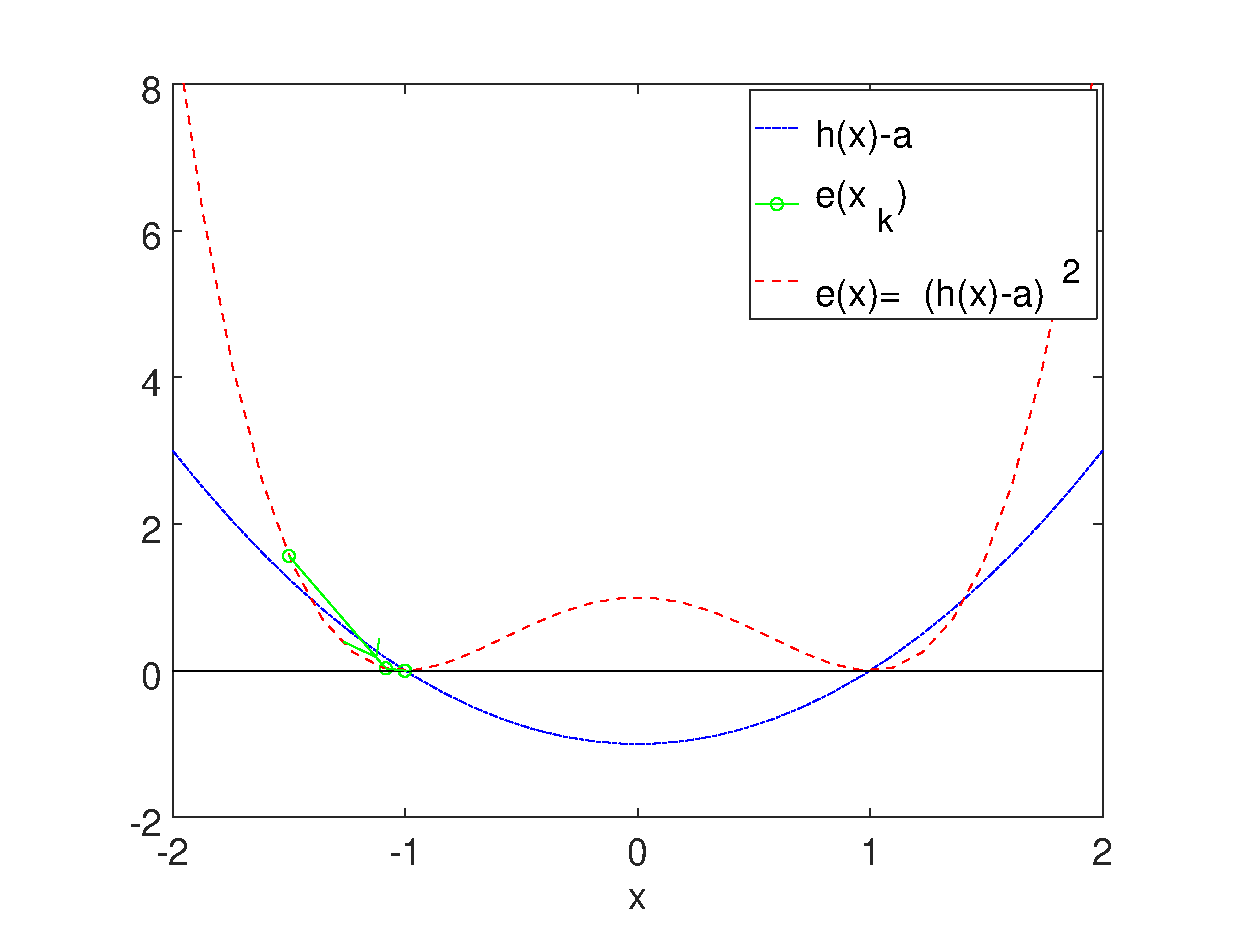
\includegraphics[width=\textwidth]{chapters/minimization/mfiles/hx_a/minimizando_hx_a_1.eps}
        \caption{Usando $h(x)=x^2$ e $a=1$, as iterações convergem}
        \label{fig:hxacasesa}
    \end{subfigure}
    ~ %add desired spacing between images, e. g. ~, \quad, \qquad, \hfill etc. 
      %(or a blank line to force the subfigure onto a new line)
    \begin{subfigure}[b]{0.45\textwidth}
        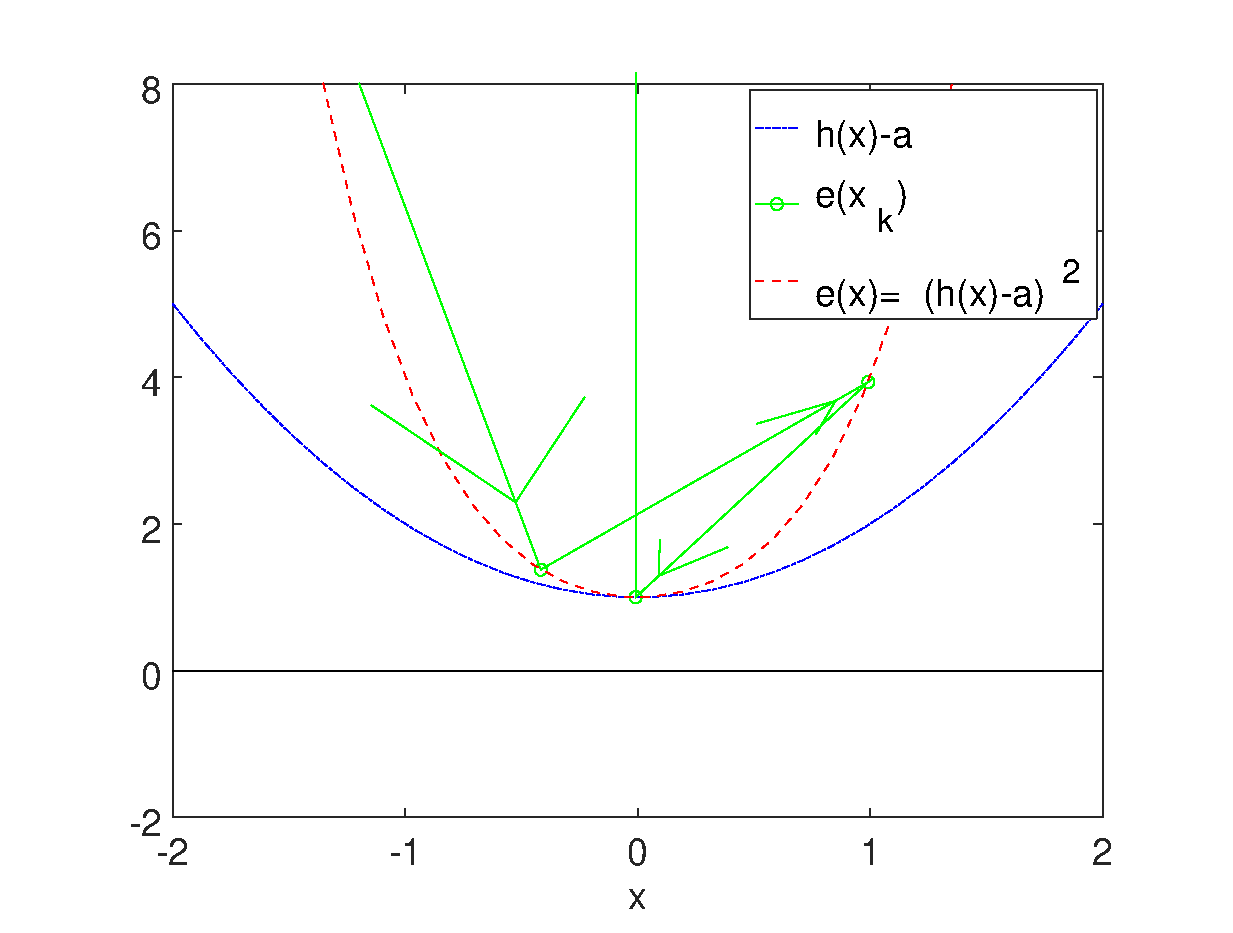
\includegraphics[width=\textwidth]{chapters/minimization/mfiles/hx_a/minimizando_hx_a_2.eps}
        \caption{Usando $h(x)=x^2$ e $a=-1$, as iterações divergem}
        \label{fig:hxacasesb}
    \end{subfigure}
    \caption{Comportamento para $h(x)=x^2$ da equação iterativa do Teorema \ref{theo:minhxhx}}
    \label{fig:hxacases}
\end{figure}

\begin{example}\label{ex:minhxhx3}
 A Fig. \ref{fig:hxacases3a} nos mostra o processo de busca de um mínimo
 de $e(x)=(h(x)-a)^2$, quando $h(x)=x^3$ e $a=1$; A busca inicia em $x_0=-1.5$,
 todos os valores $x_{k}$ podem ser vistos na segunda coluna da
Tabela \ref{tab:hxacases3}. Neste caso a Eq. (\ref{eq:minhxhx2}) \textbf{diverge} em 
valores de $x_{k}$ próximos a $0$, pois provocam valores  $h'(x_{k})\cong 0$,
este valor corresponde com um ponto de inflexão de $e(x)$.

 Por outro lado, a Fig. \ref{fig:hxacases3b} nos mostra o processo de busca de um mínimo
 de $e(x)=(h(x)-a)^2$, quando $h(x)=x^3$ e $a=-1$. A busca inicia em $x_0=-1.5$,
 todos os valores de $x_{k}$ podem ser vistos na terceira coluna da
Tabela \ref{tab:hxacases3}. Neste caso a Eq. (\ref{eq:minhxhx2}) \textbf{converge} 
em $\hat{x}=-1$ com $e(\hat{x})=0$, sendo este um mínimo absoluto.
\begin{table}[!h]
\centering
\begin{tabular}{|l|l|l|}
\hline
~&$e(x)=(x^3-1)^2$ & $e(x)=(x^3+1)^2$ \\ \hline
$k$&$x_k$  & $x_k$ \\ \hline
0&-1.50000  & -1.5000   \\
1&-0.85185  & -1.1481   \\
2&-0.10854  & -1.0183   \\
3&28.21988  & -1.0003   \\
4&18.81368  & -1.0000   \\  \hline
\end{tabular}
\caption{Convergência para $h(x)=x^3$ da equação iterativa do Teorema \ref{theo:minhxhx}}
\label{tab:hxacases3}
\end{table}
\end{example}

\begin{figure}[!h]
    \centering
    \begin{subfigure}[b]{0.45\textwidth}
        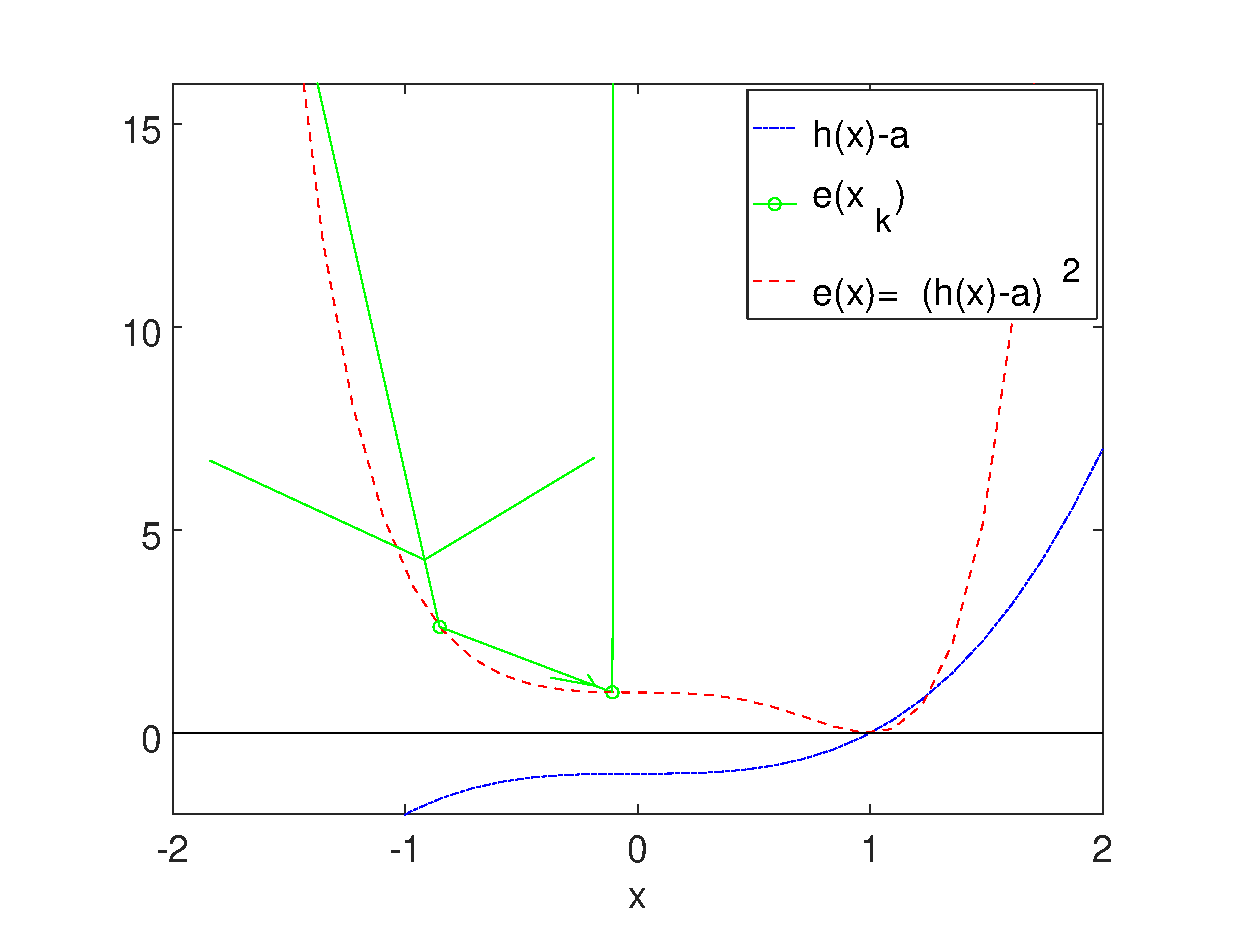
\includegraphics[width=\textwidth]{chapters/minimization/mfiles/hx3_a/minimizando_hx_a_1.eps}
        \caption{Usando $h(x)=x^3$ e $a=1$, as iterações divergem}
        \label{fig:hxacases3a}
    \end{subfigure}
    ~ %add desired spacing between images, e. g. ~, \quad, \qquad, \hfill etc. 
      %(or a blank line to force the subfigure onto a new line)
    \begin{subfigure}[b]{0.45\textwidth}
        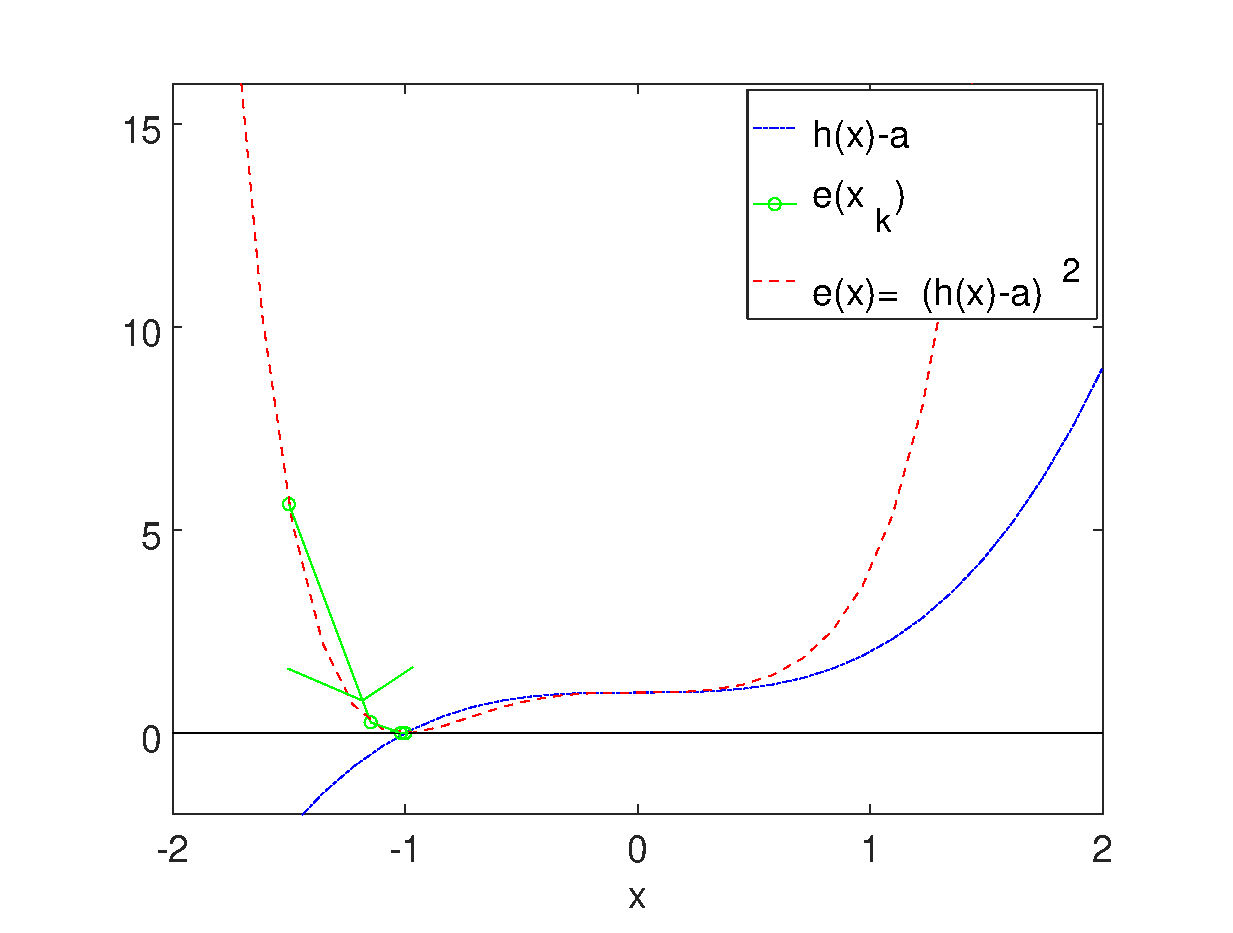
\includegraphics[width=\textwidth]{chapters/minimization/mfiles/hx3_a/minimizando_hx_a_2.eps}
        \caption{Usando $h(x)=x^3$ e $a=-1$, as iterações convergem}
        \label{fig:hxacases3b}
    \end{subfigure}
    \caption{Comportamento para $h(x)=x^3$ da equação iterativa do Teorema \ref{theo:minhxhx}}
    \label{fig:hxacases3}
\end{figure}

\index{Minimização, métodos!Método de Newton}
\index{Minimização, métodos!Regularização de Tikhonov}
\index{Problema inverso!Não linear}
\index{Minimização do erro quadrático!Não linear}

%%%%%%%%%%%%%%%%%%%%%%%%%%%%%%%%%%%%%%%%%%%%%%%%%%%%%%%%%%%%%%%%%%%%%%%%%%%%%%%%%%%%%%%
%%%%%%%%%%%%%%%%%%%%%%%%%%%%%%%%%%%%%%%%%%%%%%%%%%%%%%%%%%%%%%%%%%%%%%%%%%%%%%%%%%%%%%%
%%%%%%%%%%%%%%%%%%%%%%%%%%%%%%%%%%%%%%%%%%%%%%%%%%%%%%%%%%%%%%%%%%%%%%%%%%%%%%%%%%%%%%%
~\\
~\\
\section{\textcolor{blue}{Minimização de $||h(x)-a||^2+\alpha ||x-b||^2$}}

\begin{theorem}[Solução iterativa]\label{theo:minhxhxxbxb}
Dados,
um escalar $\alpha \in \mathbb{R} | \alpha > 0$, 
um escalar $x \in \mathbb{R}$, 
um escalar $a \in \mathbb{R}$,  
uma função $h:\mathbb{R} \rightarrow \mathbb{R}$, e 
definida a Eq. (\ref{eq:minhxhxxbxb1}),
\begin{equation}\label{eq:minhxhxxbxb1}
e(x)=||h(x)-a||^2+\alpha ||x-b||^2.
\end{equation}

Se desejamos ter o valor $\hat{x}$ que minimiza o escalar $e(\hat{x})$,
este valor pode ser achado usando iterativamente a Eq. (\ref{eq:minhxhxxbxb2}),
onde  $h'(x)\equiv \frac{\partial h(x)}{\partial x}$,
\begin{equation}\label{eq:minhxhxxbxb2}
x_{k+1} \leftarrow x_k-
\frac{ h'(x_k) \left[h(x_k)-a\right]+\alpha\left[ x_k-b\right]}{\left[h'(x_k)\right]^2+\alpha}
\end{equation}.

Assim, $\hat{x}$ pode ser achado iniciando a Eq. (\ref{eq:minhxhxxbxb2}) desde um 
$x_{0}$ qualquer, 
\begin{itemize}
    \item ate que $x_{k}$ seja muito próximo a $x_{k-1}$ (convergência de $x_{k}$) ou
    \item ate que $h(x_{k})$ seja muito próximo a $a$, 
    se conhecemos que esta igualdade é possível,
\end{itemize}
onde pode ser declarado que $\hat{x} \approx x_{k}$.\\

No processo de busca, podemos ter 3 diferentes casos:
\begin{itemize}
\item \textbf{Quando $x_{k}$ converge:}  
Se a Eq. (\ref{eq:minhxhxxbxb2}),  converge a um valor $\hat{x}$, então este se trata de 
um mínimo, relativo ou absoluto, ou ponto de inflexão de $e(x)$. 
Ver Prova \ref{proof:theo:minhxhxxbxb} e Exemplo \ref{ex:minhxhxxbxb}.
\'E importante ressaltar que quanto maior seja o valor de $\alpha$ maior
será a diferencia do ponto mínimo de $e(x)$ e $(h(x)-a)^2$.


\item \textbf{Quando $x_{k}$ diverge:}  
Acontece quando $h'(x) \approx 0$ e o fator $0<\alpha<\lim\limits_{\varepsilon \rightarrow +0}\varepsilon$, 
ver Exemplo \ref{ex:minhx3hx3xbxb}; pois quando se está perto
de um ponto crítico a busca diverge. \\
\end{itemize}

Para reconhecer o tipo de ponto crítico de $e(x)$, e souber se 
a busca debe ser continuada desde outro ponto, 
podemos seguir vários procedimentos; por exemplo, estudar o comportamento 
de $e(x_k)$ e/ou analisar  $\frac{\partial^2 e(x)}{\partial x^2}$ avaliada em $x_k$.

Uma forma de iterar, como a vista na Eq (\ref{eq:minhxhxxbxb2}) é conhecida como 
método de regularização de Tikhonov.
A demostração pode ser vista na Prova \ref{proof:theo:minhxhxxbxb}.
\end{theorem}




\begin{example}\label{ex:minhxhxxbxb}
 A Fig. \ref{fig:hxbcasesa} nos mostra o processo de busca de um mínimo
 de $e(x)=(h(x)-a)^2+\alpha (x-b)^2$, quando $h(x)=x^2(x^2-1)$, $a=1$, $b=0$ e $\alpha=1.2$. A busca inicia em $x_0=-1.4$,
 todos os valores $x_{k}$ podem ser vistos na segunda coluna da
Tabela \ref{tab:hxbcases}. Neste caso a Eq. (\ref{eq:minhxhxxbxb2}) \textbf{converge} sem problemas 
em $\hat{x}=-1.21239$ com $e(\hat{x})=1.85954$; porem, 
 este valor de $x$ está longe do mínimo
 absoluto de  $e(x)$ que está em $e(x=0)=1.0$; por outro lado, este valor de $x$
 está perto do mínimo absoluto de  $(h(x)-a)^2$, que está em 
 $x=\pm\sqrt{\frac{1+\sqrt{5}}{2}}\approx \pm1.2720$. Isto é consequência do uso do fator 
 $\alpha>0$, pelo qual é de esperar que quanto maior seja o valor de $\alpha$
 maior será a diferencia do mínimo absoluto de $e(x)$ e de $(h(x)-a)^2$.

 A Fig. \ref{fig:hxbcasesb} nos mostra o processo de busca de um mínimo
 de $e(x)=(h(x)-a)^2+\alpha (x-b)^2$, quando $h(x)=x^2(x^2-1)$, $a=-1$, $b=0$ e $\alpha=1.2$. A busca inicia em $x_0=-1.4$,
 todos os valores $x_{k}$ podem ser vistos na terceira coluna da
Tabela \ref{tab:hxbcases}. Neste caso a Eq. (\ref{eq:minhxhxxbxb2}) \textbf{converge} 
em $\hat{x}=-0.39349$ com $e(\hat{x})=0.94120$ que é o mínimo absoluto de $e(x)$; porem, este valor de $x_k$ está
um pouco distante do mínimo de $(h(x)-a)^2$, localizado em $x=\pm\frac{\sqrt{2}}{2}\approxeq \pm0.70711$.
Novamente, isto é consequência do uso do fator 
 $\alpha>0$, assim, quanto maior seja o valor de $\alpha$
 maior será a diferencia do mínimo absoluto de $e(x)$ e de $(h(x)-a)^2$.

\begin{table}[!h]
\centering
\begin{tabular}{|l|l|l|}
\hline
~&$e(x)=(x^2(x^2-1)-1)^2+1.2x^2$ & $e(x)=(x^2(x^2-1)+1)^2+1.2x^2$ \\ \hline
$k$&$x_k$  & $x_k$ \\ \hline
0&-1.4000  & -1.40000     \\
1&-1.2694  & -1.02908     \\
2&-1.2258  & -0.46252     \\
3&-1.2153  & -0.38498     \\
4&-1.2130  & -0.39259     \\  
5&-1.2125  & -0.39341     \\  
6&-1.2124  & -0.39348     \\ 
7&-1.2124  & -0.39349     \\ \hline
\end{tabular}
\caption{Convergência para $h(x)=x^2(x^2-1)$ da equação iterativa do Teorema \ref{theo:minhxhxxbxb}}
\label{tab:hxbcases}
\end{table}
\end{example}

\begin{figure}[!h]
    \centering
    \begin{subfigure}[b]{0.45\textwidth}
        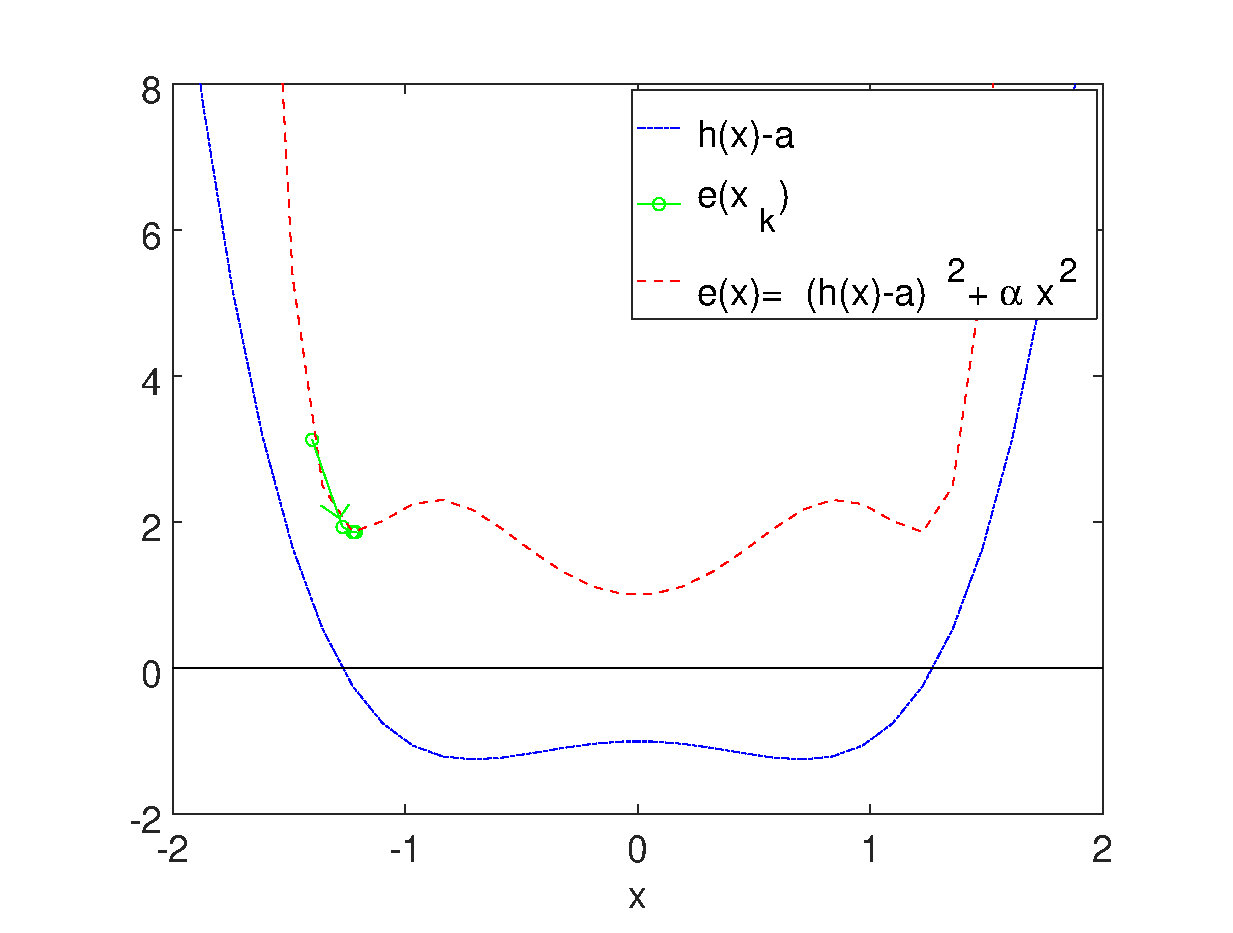
\includegraphics[width=\textwidth]{chapters/minimization/mfiles/hx_a_alphax/minimizando_hx_a_alphax_1.eps}
        \caption{Usando $h(x)=x^2(x^2-1)$, $a=1$, $b=0$ e $\alpha=1.2$, as iterações convergem}
        \label{fig:hxbcasesa}
    \end{subfigure}
    ~ %add desired spacing between images, e. g. ~, \quad, \qquad, \hfill etc. 
      %(or a blank line to force the subfigure onto a new line)
    \begin{subfigure}[b]{0.45\textwidth}
        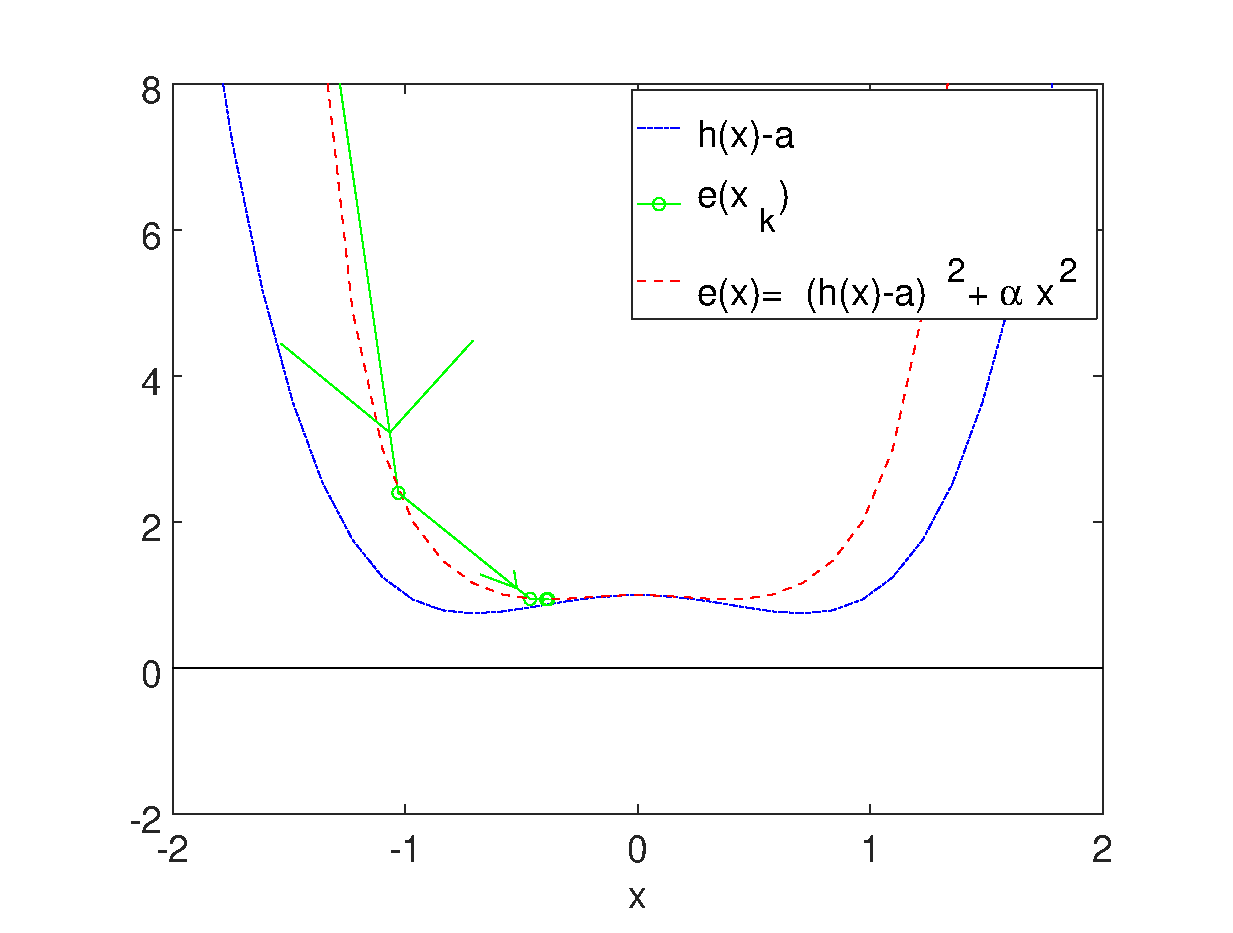
\includegraphics[width=\textwidth]{chapters/minimization/mfiles/hx_a_alphax/minimizando_hx_a_alphax_2.eps}
        \caption{Usando $h(x)=x^2(x^2-1)$, $a=-1$, $b=0$ e $\alpha=1.2$, as iterações convergem}
        \label{fig:hxbcasesb}
    \end{subfigure}
    \caption{Comportamento para $h(x)=x^2(x^2-1)$ da equação iterativa do Teorema \ref{theo:minhxhxxbxb}}
    \label{fig:hxbcases}
\end{figure}



\begin{example}\label{ex:minhx3hx3xbxb}
 A Fig. \ref{fig:hx3bcasesa} nos mostra o processo de busca de um mínimo
 de $e(x)=(h(x)-a)^2+\alpha (x-b)^2$, quando $h(x)=(x+0.5)^3$, $a=1$, $b=0$ e $\alpha=0.01$. 
 A busca inicia em $x_0=-1.4$,
 todos os valores $x_{k}$ podem ser vistos na segunda coluna da
Tabela \ref{tab:hx3bcases}. Neste caso a Eq. (\ref{eq:minhxhxxbxb2}) num principio \textbf{diverge}
em pontos próximos a $x=-0.5$, apos a divergência, as iterações continuam desde 
$x=+4.665$ e estas \textbf{convergem} sem problemas 
em $\hat{x}=+0.53255$ com $e(\hat{x})\approx 0.013$; este valor de $x$
 está perto do mínimo absoluto de  $(h(x)-a)^2$, que está em 
 $x=+0.5$. Isto é consequência do uso do fator 
 $\alpha>0$ e pequeno, pelo qual é de esperar que quanto maior seja o valor de $\alpha$
 maior será a diferencia do mínimo absoluto de $e(x)$ e de $(h(x)-a)^2$.

 A Fig. \ref{fig:hx3bcasesb} nos mostra o processo de busca de um mínimo
 de $e(x)=(h(x)-a)^2+\alpha (x-b)^2$, quando $h(x)=(x+0.5)^3$, 
 $a=1$, $b=0$ e $\alpha=1.2$. A busca inicia em $x_0=-1.4$,
 todos os valores $x_{k}$ podem ser vistos na terceira coluna da
Tabela \ref{tab:hx3bcases}. Neste caso a Eq. (\ref{eq:minhxhxxbxb2}) \textbf{converge} 
em $\hat{x}=+0.428757$ com $e(\hat{x})\approx 0.26$,
que é o mínimo absoluto de $e(x)$; porem, este valor de $x_k$ está
um pouco distante do mínimo de $(h(x)-a)^2$, localizado em $x=+0.5$.
Novamente, isto é consequência do uso do fator 
 $\alpha>0$ e grande.

\begin{table}[!h]
\centering
\begin{tabular}{|l|l|l|}
\hline
~&$e(x)=((x+0.5)^3-1)^2+0.01x^2$ & $e(x)=((x+0.5)^3+1)^2+1.2x^2$ \\ \hline
$k$&$x_k$  & $x_k$ \\ \hline
0&-1.40000  &-1.40000     \\
1&-0.68731  &-0.572195      \\
2&+4.66500  &+0.012916      \\
3&+2.95583  &+0.378950      \\
4&+1.83178  &+0.422950      \\  
5&+1.11578  &+0.427972      \\  
6&+0.70475  &+0.428660      \\ 
7&+0.53255  &+0.428757      \\ \hline
\end{tabular}
\caption{Convergência para $h(x)=(x+0.5)^3$ da equação iterativa do Teorema \ref{theo:minhxhxxbxb}}
\label{tab:hx3bcases}
\end{table}
\end{example}

\begin{figure}[!h]
    \centering
    \begin{subfigure}[b]{0.45\textwidth}
        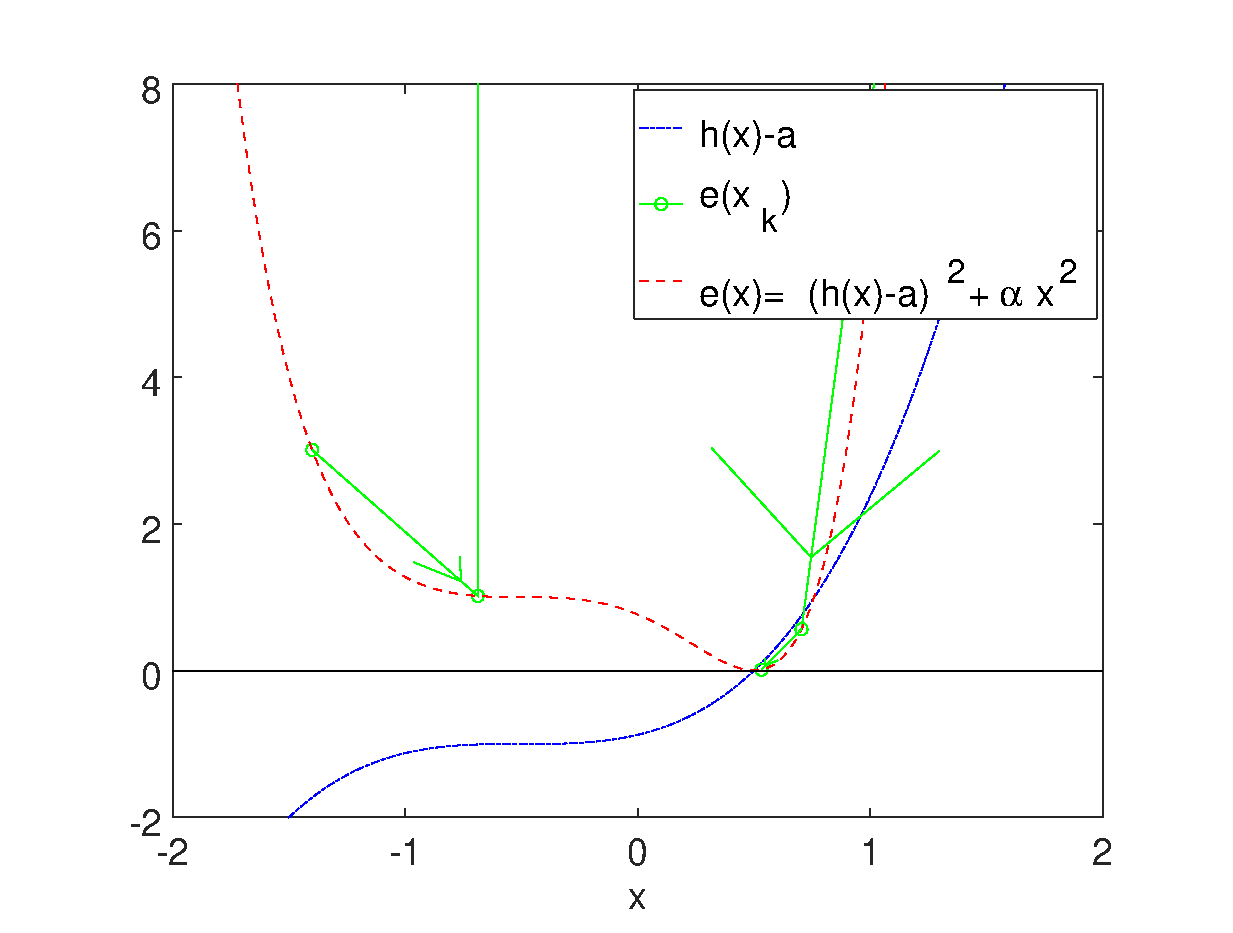
\includegraphics[width=\textwidth]{chapters/minimization/mfiles/hx3_a_alphax/minimizando_hx_a_alphax_1.eps}
        \caption{Usando $h(x)=(x+0.5)^3$, $a=1$ e $\alpha=0.01$, as iterações divergem e logo convergem}
        \label{fig:hx3bcasesa}
    \end{subfigure}
    ~ %add desired spacing between images, e. g. ~, \quad, \qquad, \hfill etc. 
      %(or a blank line to force the subfigure onto a new line)
    \begin{subfigure}[b]{0.45\textwidth}
        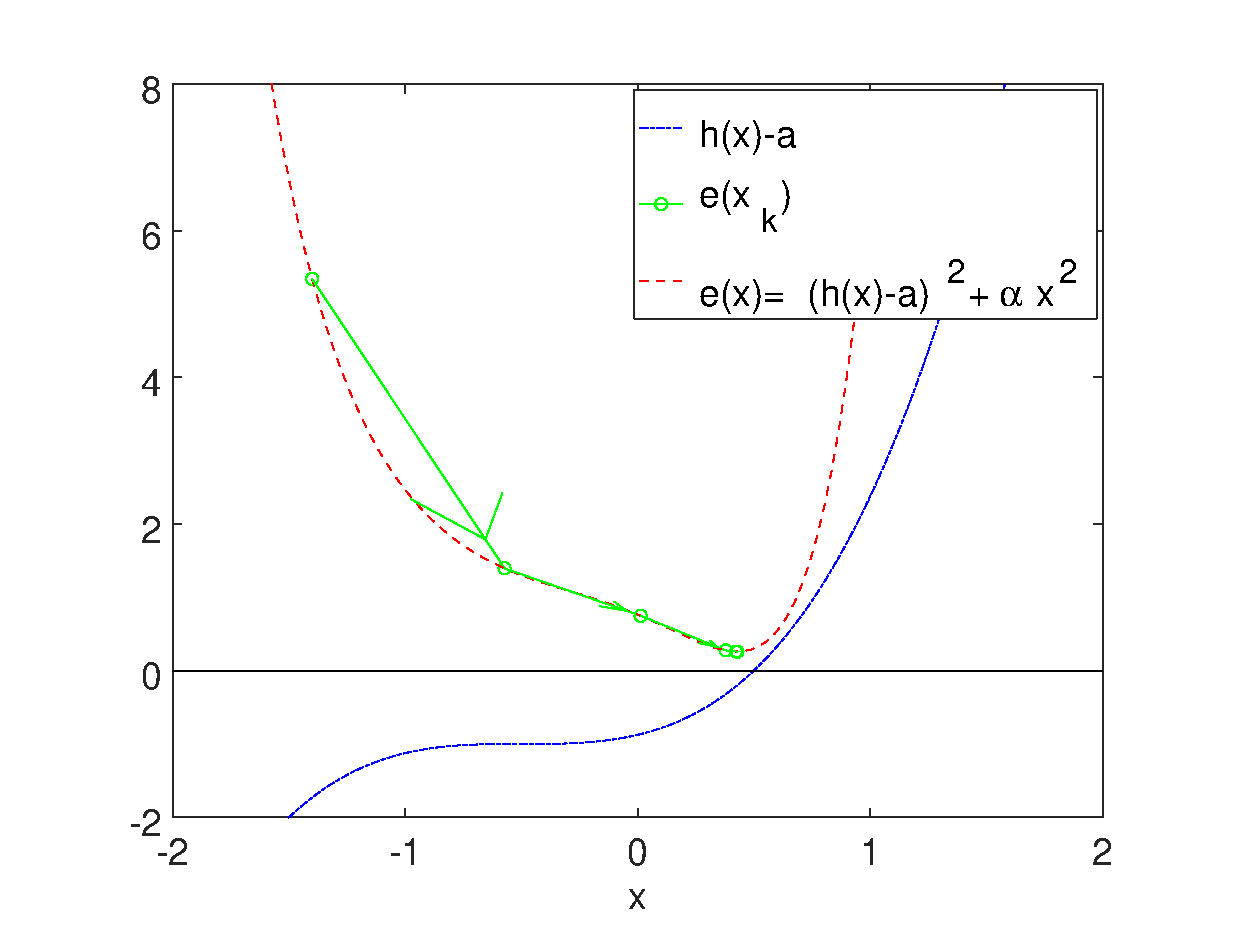
\includegraphics[width=\textwidth]{chapters/minimization/mfiles/hx3_a_alphax/minimizando_hx_a_alphax_2.eps}
        \caption{Usando $h(x)=(x+0.5)^3$, $a=1$ e $\alpha=1.2$, as iterações convergem no mínimo absoluto}
        \label{fig:hx3bcasesb}
    \end{subfigure}
    \caption{Comportamento para $h(x)=(x+0.5)^3$ da equação iterativa do Teorema \ref{theo:minhxhxxbxb}}
    \label{fig:hx3bcases}
\end{figure}
%%%%%%%%%%%%%%%%%%%%%%%%%%%%%%%%%%%%%%%%%%%%%%%%%%%%%%%%%%%%%%%%%%%%%%%%%%%%%%%%%%%%%%%
%%%%%%%%%%%%%%%%%%%%%%%%%%%%%%%%%%%%%%%%%%%%%%%%%%%%%%%%%%%%%%%%%%%%%%%%%%%%%%%%%%%%%%%
%%%%%%%%%%%%%%%%%%%%%%%%%%%%%%%%%%%%%%%%%%%%%%%%%%%%%%%%%%%%%%%%%%%%%%%%%%%%%%%%%%%%%%%
\section{\textcolor{blue}{Minimização de $||h(x)-a||^2+\alpha ||x-x_{old}||^2$}}

\begin{theorem}[Solução iterativa]\label{theo:minhxhxxoxo}
Dados,
um escalar $\alpha \in \mathbb{R} | \alpha > 0$, 
um escalar $x \in \mathbb{R}$, 
um escalar $a \in \mathbb{R}$,  
uma função $h:\mathbb{R} \rightarrow \mathbb{R}$, e 
definida a Eq. (\ref{eq:minhxhxxoxo1}),
\begin{equation}\label{eq:minhxhxxoxo1}
e(x)=||h(x)-a||^2+\alpha ||x-x_{old}||^2.
\end{equation}
Se desejamos ter o valor $\hat{x}$ que minimiza o escalar $e(\hat{x})$,
este valor pode ser achado usando iterativamente a Eq. (\ref{eq:minhxhxxoxo2}),
\begin{equation}\label{eq:minhxhxxoxo2}
x_{k+1} \leftarrow x_k+
\frac{ h'(x_k) \left[a-h(x_k)\right] }{\left[h'(x_k)\right]^2+\alpha}
\end{equation}
Onde  $h'(x)=\frac{\partial h(x)}{\partial x}$.
Assim, $\hat{x}$ pode ser achado iniciando a Eq. (\ref{eq:minhxhxxoxo2}) desde um $x_{0}$ qualquer, ate que $x_{k}$ seja muito próximo a $x_{k+1}$,
onde se declara que $\hat{x} \approx x_{k+1}$; porem deve ser corroborado
que esse ponto tratasse de um máximo ou mínimo usando algum método, por exemplo estudando o comportamento 
de $e(x)$ ou analisando  $\frac{\partial^2 e(x)}{\partial x^2}$ avaliada em $\hat{x}$.

\FALTAPROVA
A demostração pode ser vista na Prova \ref{proof:theo:minhxhxxoxo}.
\end{theorem}

